\subsection{Адаптивный рандомизированный\\ жадный алгоритм (ARG)}
\label{sub:arg}


\subsubsection*{Применимость алгоритма SPSA}
\label{ssub:spsa_validity}

Применимость \emph{SPSA} обоснована теоретически для выпуклой усредненной функции качества.

В зависимости от графа модулярность результатов работы $RG_k$ либо принимает максимум при небольшом $k$, как на рисунке \ref{fig:spsa_validity_karate}, либо постепенно увеличивается при росте $k$, как на рисунке \ref{fig:spsa_validity_netscience}.

\begin{figure}[h!]
	\centering
	\begin{subfigure}{.45\textwidth}
		\centering
		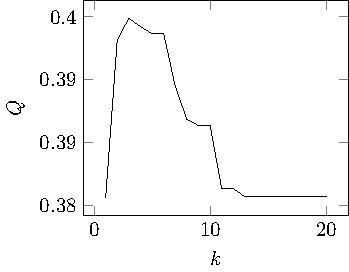
\includegraphics[width=\linewidth]{prodanov/prodanov_validity_karate.eps}
		\caption{Зависимость модулярности от $k$ на графе \emph{karate}}
		\label{fig:spsa_validity_karate}
	\end{subfigure}
	%
	\begin{subfigure}{.1\textwidth}
	\end{subfigure}
	%
	\begin{subfigure}{.45\textwidth}
		\centering
		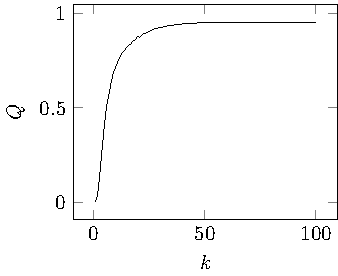
\includegraphics[width=\linewidth]{prodanov/prodanov_validity_netscience.eps}
		\caption{Зависимость модулярности от $k$ на графе \emph{netscience}}
		\label{fig:spsa_validity_netscience}
	\end{subfigure}
\caption{Зависимость модулярности от параметра $k$ на двух графах}
\label{fig:spsa_validity}
\end{figure}

Значение $k$, при которым $RG_k$ будет на графе принимать наилучшее значение, далее в работе называется \emph{оптимальным} $k$ или $k_{opt}$.

Время работы $RG_k$ линейно растёт при росте $k$, поэтому